\section{Additional figure}


\begin{figure}[!htbp]
\centering
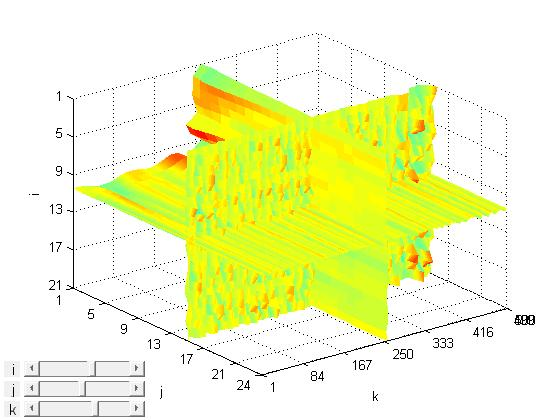
\includegraphics[width=1\textwidth]{16.jpg}
\caption{Individual component of the hsvd of the water filtered signal}
\end{figure}

\begin{figure}[!htbp]
\centering
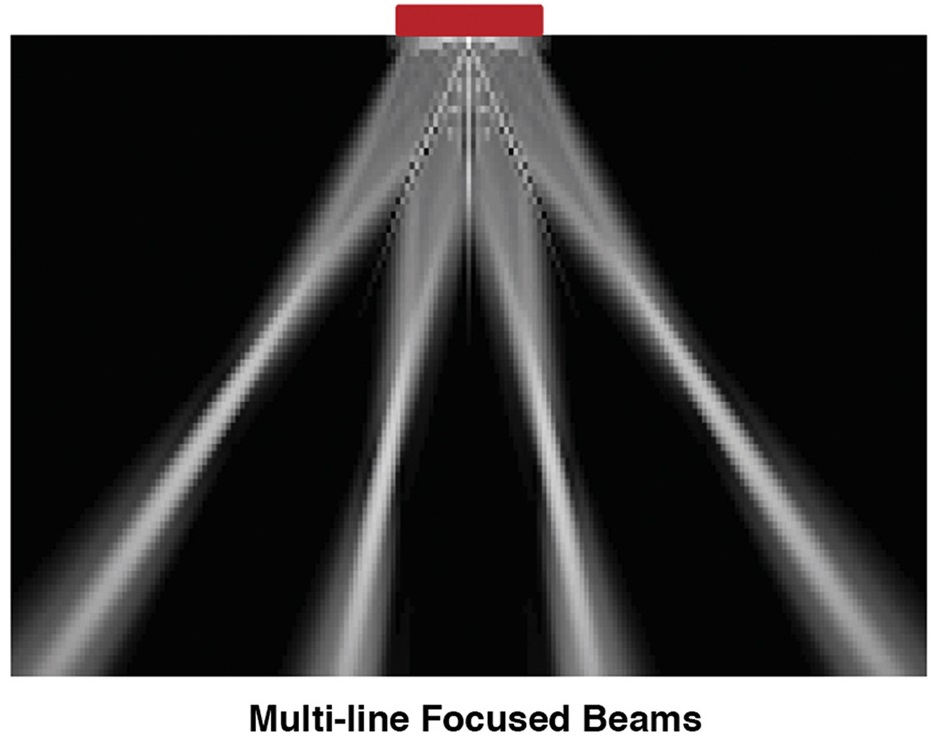
\includegraphics[width=1\textwidth]{17.jpg}
\caption{Individual component of the hsvd of the noisy water filtered signal}
\end{figure}

\begin{figure}[!htbp]
\centering
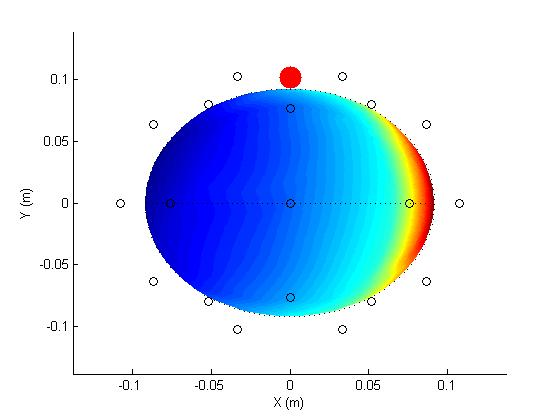
\includegraphics[width=1\textwidth]{18.jpg}
\caption{Individual component of the htlsU of the water filtered signal}
\end{figure}

\begin{figure}[!htbp]
\centering
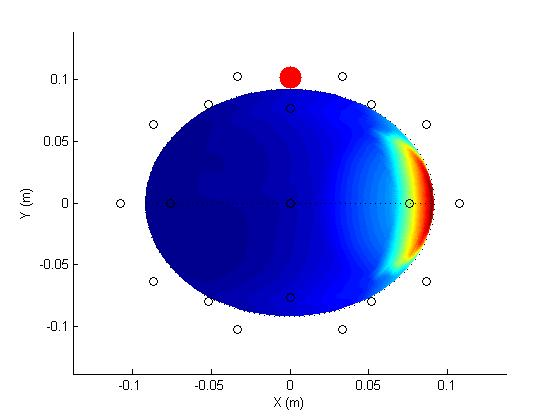
\includegraphics[width=1\textwidth]{19.jpg}
\caption{Individual component of the htlsU of the noisy water filtered signal}
\end{figure}

\begin{figure}[!htbp]
\centering
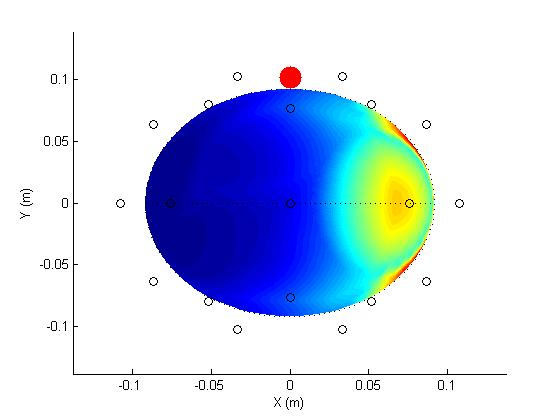
\includegraphics[width=1\textwidth]{20.jpg}
\caption{Individual component of the htlspkfd of the water filtered signal}
\end{figure}

\begin{figure}[!htbp]
\centering
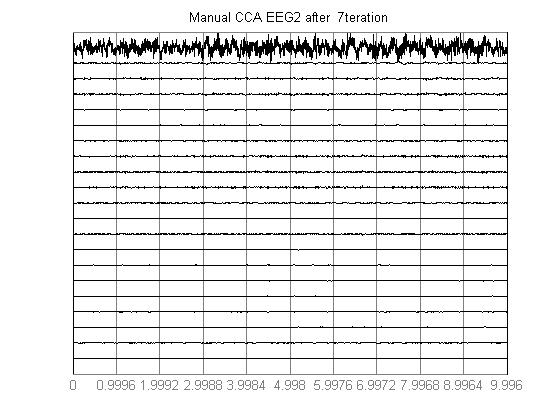
\includegraphics[width=1\textwidth]{21.jpg}
\caption{Individual component of the htlspkfd of the noisy water filtered signal}
\end{figure}



\begin{figure}[!htbp]
\minipage{.5\textwidth}%
\centering
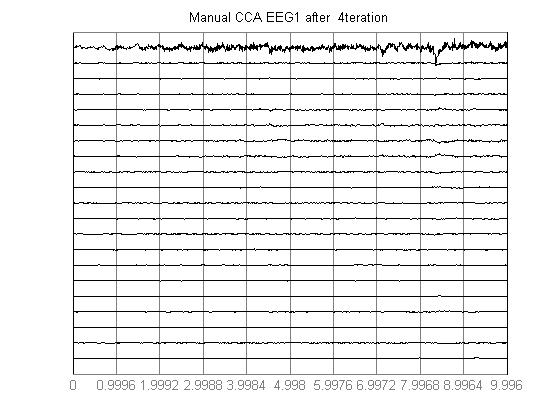
\includegraphics[width=1\textwidth]{12.jpg}
\subcaption{}
\endminipage\hfill
\minipage{.5\textwidth}%
\centering
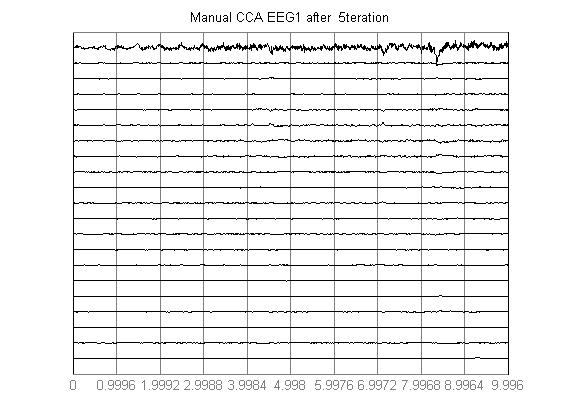
\includegraphics[width=1\textwidth]{13.jpg}
\subcaption{}
\endminipage\hfill
\minipage{.5\textwidth}%
\centering
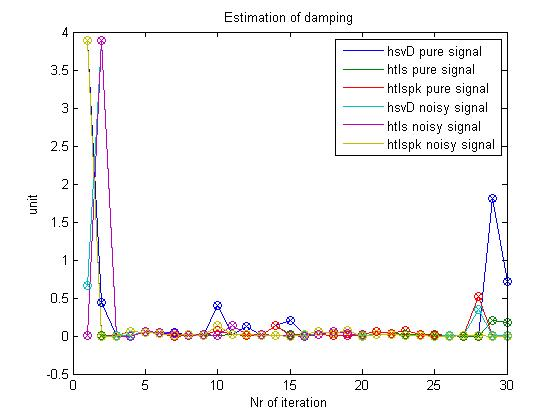
\includegraphics[width=1\textwidth]{14.jpg}
\subcaption{}
\endminipage\hfill
\minipage{.5\textwidth}%
\centering
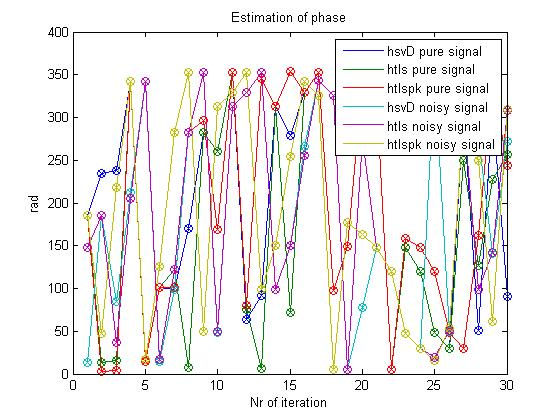
\includegraphics[width=1\textwidth]{15.jpg}
\subcaption{}
\endminipage\hfill
\caption{}
\end{figure}






